\section{DevOps cycle and practices} DevOps concepts reflect in a set of practices during the DevOps delivery cycle. The cycle is visualized in Figure 2.1. These practices mainly represent the automation concept but also come together with other concepts.\cite{devops-principles}

\begin{figure}[h]
\centering
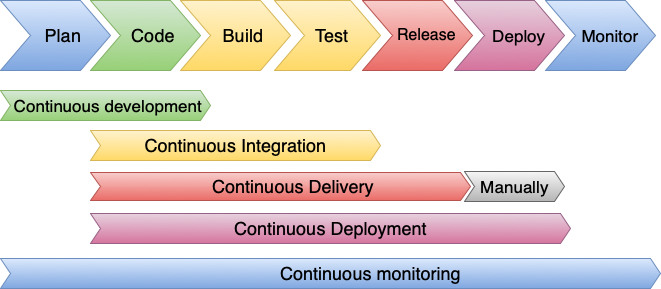
\includegraphics[scale=0.56]{../png/devops.png}
\caption{Devops cycle and practices}\label{picture:devops}
\end{figure}

\subsection{Continuous development} Continuous development is a practice composed of agile planning and coding. The goal of agile planning  is to divide big problems into smaller logical problems, estimate the complexity of created tasks and plan the amount of tasks for some short time period(sprint), usually it is from one to four weeks period. This method allows getting some large significant tasks done in a shorter time, because after its division developers can work on the subtasks simultaneously and it is more effortless for testing.

\subsection{Continuous integration (CI)} In order to avoid a problem with the integration of large parts of code, DevOps CI offers continuous pushing the code changes to the remote shared repository on the server. Every change pushed to the repository triggers a build and tests configured in a CI pipeline to make sure new changes do not affect already functioning features and also does not contain new errors.

\subsection{Continuous delivery (CD)} Continuous delivery is an extension of continuous integration. After building and testing the code from the repository it automatically deploys releases to the testing environment and also prepares it to be deployed to the production. It requires human intervention to deploy a release to production. This is a safer version of fast and frequent deployment, in a case when the pipeline does not contain strong testing tools and the application needs to be tested manually.

\subsection{Continuous deployment (CDE)} Coupled with continuous delivery, the continuous deployment also deploys the release to the production. Using this practice no human intervention is required. Every change pushed to the main shared remote repository will be automatically deployed to production. The only obstacle to the deployment would be a failed build or test.

\subsection{Continuous monitoring (CM)} Continuous monitoring is an automated method that allows to observe and discover compliance concerns and security vulnerabilities throughout the DevOps lifecycle. It also finalizes the cycle by providing feedback on monitoring and informing about existing or possible failures. It helps to resolve issues in real-time.

\subsection{Infrastructure as Code (IaC)} Infrastructure as a code is a practice of managing infrastructure that enables automation in the DevOps lifecycle. It offers using scripts for configuring deployment environment and other infrastructure, including establishing a version control system.

\subsection{Containerization} Containerization is the practice of packaging an application in one container. It provides better flexibility for deployment and needs fewer resources to run. Currently, Docker provides the most frequently used container toolset.
% https://www.docker.com
